\documentclass[11pt,a4paper]{article}
\usepackage[T1]{fontenc}
\usepackage[utf8]{inputenc}
\usepackage{lmodern}
\usepackage[margin=2.5cm]{geometry}
\usepackage{graphicx}
\usepackage{booktabs}
\usepackage{amsmath}
\usepackage{siunitx}
\usepackage[numbers,sort&compress]{natbib}
\usepackage[hidelinks]{hyperref}
\hypersetup{pdftitle={When the Reference Is Extracted: TextRank Outscores Fine-Tuned Transformers and a Small LLM on BBC News Summary},pdfauthor={Muzammal Hussain}}
\usepackage{xcolor}
\usepackage{caption}
\captionsetup{font=small,labelfont=bf}
\sisetup{detect-all}

\title{When the Reference Is Extracted: TextRank Outscores Fine-Tuned Transformers and a Small LLM on BBC News Summary}
\author{Muzammal Hussain\\
\small Independent researcher, Glasgow, United Kingdom\\
\small \href{mailto:muzammal@masmatixinnovations.co.uk}{muzammal@masmatixinnovations.co.uk}\\
\small ORCID: \href{https://orcid.org/0009-0001-2570-5686}{0009-0001-2570-5686}}
\date{\small Preprint, November 2026}

\setlength{\emergencystretch}{2em}
\begin{document}
\maketitle

\begin{abstract}
BBC News Summary is a small, widely used dataset for teaching and comparing text summarisers, yet how its reference summaries were made is not documented. We audit the dataset and then compare fourteen systems on one leakage-free split: four extractive baselines, three zero-shot models, six fine-tuned encoder--decoder models and a 1.5B-parameter instruction-tuned language model adapted with LoRA, with three seeds per fine-tuned model. Of the 2,225 articles, 154 are near-duplicates; under a naive random split, 11.5\% of test articles would have a copy in training. 94.8\% of reference sentences occur verbatim in the article, and a reference is on average 45\% as long as its article. On 311 held-out articles, TextRank given the training-set length ratio scores 82.9 ROUGE-Lsum and 77.3 ROUGE-2, ahead of the best fine-tuned model, PEGASUS-large (72.7 and 64.5; paired difference $+10.2$, 95\% CI 8.7--11.5), and higher on 81\% of articles; the gap persists on BERTScore. Every fine-tuned model beats a length-matched Lead baseline on ROUGE-2, but Flan-T5-base and Flan-T5-large do not on ROUGE-Lsum, and Flan-T5-large, which writes the shortest summaries, scores below its smaller sibling. Zero-shot models score 25--38 ROUGE-Lsum, mostly because of length and wording, and the zero-shot LLM writes numbers absent from the article (7.8\% of its numbers, 0.8\% after LoRA). We conclude that BBC News Summary mainly measures how well a system reproduces a sentence-selection rule, and that results on it should always be reported next to a length-matched TextRank baseline. Code, splits, per-document scores and the Kaggle notebook are public.
\end{abstract}

\section{Introduction}
Summarisation benchmarks are only as informative as their references. Large news corpora such as CNN/DailyMail \cite{hermann2015cnndm} and Newsroom \cite{grusky2018newsroom} are known to reward copying and lead position \cite{kryscinski2019critical,jung2019earlier}, and automatic metrics track human judgement only partly \cite{fabbri2021summeval}. Smaller datasets receive less scrutiny. BBC News Summary \cite{pariza2018bbcsum}, built on the BBC articles of \citet{greene2006bbc}, pairs 2,225 articles from 2004--2005 with one summary each and is a common choice in coursework, tutorials and applied papers, often to compare fine-tuned transformers.

This study began as a rebuild of an earlier project of the author's that fine-tuned five transformers on this dataset. A code review found that the earlier pipeline had trained on swapped columns (summary in, article out), reversed the ROUGE arguments and evaluated on rows that overlapped training. Its scores were withdrawn. Rather than repeat the comparison, we first asked what the references are, and then compared models under a protocol designed to avoid those errors.

Our contributions are:
\begin{enumerate}
  \item An audit of BBC News Summary: near-duplicates, the leakage they cause under random splits, and how extractive and lead-biased the references are (Section~\ref{sec:audit}).
  \item A leakage-free comparison of fourteen systems on a fixed, published split, with three seeds, bootstrap intervals and paired tests (Sections~\ref{sec:setup}--\ref{sec:results}).
  \item The finding that a training-free, length-matched TextRank \cite{mihalcea2004textrank} outscores all fine-tuned models, with an analysis of why: output form, length and the apparent selection rule behind the references (Section~\ref{sec:discussion}).
\end{enumerate}

\section{Related work}
\citet{kryscinski2019critical} showed that common news benchmarks are dominated by layout bias and that ROUGE rewards extractive overlap; \citet{jung2019earlier} quantified position, diversity and importance biases across corpora; \citet{grusky2018newsroom} introduced coverage, density and compression to describe how extractive a summary is, which we use here. SummEval \cite{fabbri2021summeval} re-evaluated metrics against human ratings. With instruction-tuned LLMs, \citet{goyal2022gpt3} and \citet{zhang2024benchmarking} found that reference summaries in standard datasets are often worse than model outputs as judged by people, so reference-based scores can mislead. Faithfulness concerns for abstractive models are surveyed by \citet{maynez2020faithfulness}. Duplicate removal before splitting is standard advice in language-model training \cite{lee2022dedup} but is rarely reported for small summarisation datasets. We are not aware of a published audit of how the BBC News Summary references were built.

\section{Dataset audit}\label{sec:audit}
\paragraph{Data.} Each article file starts with its headline, followed by the body; each summary file contains sentences from the body, concatenated without spaces between them. We repaired sentence boundaries (inserting a space after sentence-final punctuation followed by a capital letter, preserving decimals and initialisms), removed the headline from model inputs, and split text into sentences with an abbreviation-aware rule.

\paragraph{Duplicates and leakage.} Two articles are near-duplicates if the Jaccard similarity of their word 5-gram sets is at least 0.9. We found 154 near-duplicates (138 exact copies), all within the same category. In 20 random 85/15 splits of the raw data, on average 38.6 of 334 test articles (11.5\%) had a near-duplicate in training. We removed duplicates, keeping the first of each group, and used the remaining 2,071 articles.

\paragraph{How the references were built.} Table~\ref{tab:audit} summarises the references. 94.8\% of reference sentences occur verbatim (after lower-casing and removing punctuation) in the article. The median reference has 149 words against 329 for the article (compression 0.454), consistently across categories (0.446--0.465). References favour the start of the article but select throughout it: 62.5\% of sentences in the first tenth of an article are selected, falling to about 40\% in the middle and 30.8\% in the last tenth (Figure~\ref{fig:position}); 73.7\% of references include the first sentence. We found no documentation of how the references were produced; this profile, roughly the most central half of the article copied in order, is what an automatic sentence-scoring method would produce.

\begin{table}[t]
\centering\small
\caption{Audit of BBC News Summary. Verbatim: share of reference sentences found unchanged in the article. First: share of references that contain the article's first sentence.}
\label{tab:audit}
\resizebox{\linewidth}{!}{%
\begin{tabular}{lrrrrrr}
\toprule
Category & Articles & Article words & Ref.\ words & Compression & Verbatim (\%) & First (\%)\\
\midrule
Business & 500 & 295 & 134 & 0.450 & 95.8 & 78.8\\
Entertainment & 364 & 261 & 124 & 0.457 & 94.3 & 80.2\\
Politics & 394 & 441 & 195 & 0.452 & 92.1 & 66.2\\
Sport & 489 & 285 & 131 & 0.465 & 95.6 & 75.5\\
Tech & 324 & 460 & 206 & 0.446 & 95.5 & 65.1\\
\midrule
All (after de-duplication) & 2,071 & 329 & 149 & 0.454 & 94.8 & 73.7\\
\bottomrule
\end{tabular}}
\end{table}

\begin{figure}[t]
\centering
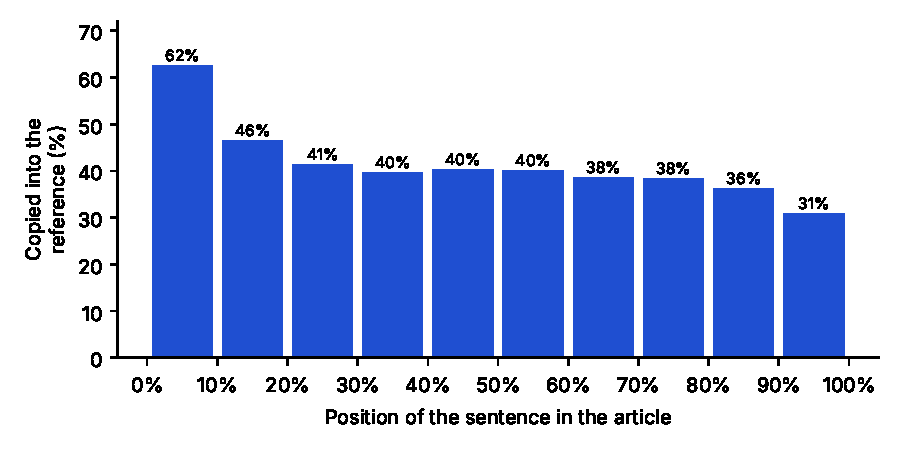
\includegraphics[width=0.72\linewidth]{figures/reference_position.pdf}
\caption{Share of article sentences copied into the reference, by relative position in the article (all 2,071 articles).}
\label{fig:position}
\end{figure}

\section{Experimental setup}\label{sec:setup}
\paragraph{Split.} After de-duplication we drew one split, stratified by category, with a fixed seed: 1,449 training, 311 validation and 311 test articles. The split file is released. The test set was used once per system, for final generation.

\paragraph{Length budget.} Several systems need a target length. We set it to $r \times$ (article words), with $r = 0.455$ the median reference-to-article length ratio on the training split. No system sees the length of the test reference.

\paragraph{Extractive baselines.} \textit{Lead-3} takes the first three sentences. \textit{Lead, length-matched} takes sentences from the start until the budget is reached. \textit{TextRank} ranks sentences by PageRank over TF-IDF cosine similarity (damping 0.85) and takes the top-ranked sentences up to the budget, output in article order. The \textit{extractive oracle} greedily adds the sentence that most increases ROUGE-1 + ROUGE-2 against the reference, and is an upper bound for sentence selection.

\paragraph{Zero-shot models.} BART-large-CNN and PEGASUS-CNN/DailyMail are summarisers fine-tuned on CNN/DailyMail \cite{lewis2020bart,zhang2020pegasus}. Qwen2.5-1.5B-Instruct \cite{qwen2025qwen25} is prompted to ``summarise the following news article in about $n$ words'' with $n$ from the length budget, and decoded greedily.

\paragraph{Fine-tuned models.} BART-base and BART-large \cite{lewis2020bart}, T5-base \cite{raffel2020t5}, Flan-T5-base and Flan-T5-large \cite{chung2024flan}, and PEGASUS-large \cite{zhang2020pegasus} are fully fine-tuned; Qwen2.5-1.5B-Instruct is fine-tuned with LoRA \cite{hu2022lora} (rank 16, $\alpha = 32$, all linear layers) on the same prompt. Inputs are truncated to 1,024 tokens and targets to 320 (400 for the LLM). Hyperparameters were fixed in advance from common practice (AdamW for BART and the LLM, Adafactor for T5 and PEGASUS; learning rates $3\times10^{-5}$ to $5\times10^{-4}$; linear schedule with 5\% warm-up) and selected checkpoints by validation loss with early stopping. Encoder--decoders decode with beam search (4 beams, no repeated trigrams). Each fine-tuned model was trained with three seeds. Training ran on NVIDIA T4 GPUs on Kaggle, in two sessions of about 18 hours wall-clock in total (31 GPU-hours).

\paragraph{Metrics.} ROUGE-1, ROUGE-2, ROUGE-L and ROUGE-Lsum F1 \cite{lin2004rouge} with stemming (Google's \texttt{rouge-score}, sentence-split input for ROUGE-Lsum); BERTScore F1 with RoBERTa-large and baseline rescaling \cite{zhang2020bertscore}; summary length; coverage, density \cite{grusky2018newsroom} and the share of novel bigrams; and the share of numbers in a summary that do not occur in the article, as a rough check of invented content. For fine-tuned models, per-article scores are averaged over seeds; we report 95\% percentile bootstrap intervals over articles (1,000 resamples) and paired bootstrap differences.

\paragraph{Topic shift.} To test generalisation across categories, BART-base was trained five more times, each time without one category, and tested on the test articles of the held-out category; we compare with the seed-0 BART-base trained on all categories, on the same articles.

\section{Results}\label{sec:results}
Table~\ref{tab:main} and Figure~\ref{fig:main} give the main results.

\begin{table}[t]
\centering\small
\caption{Results on the 311 test articles. Fine-tuned rows are means over three seeds ($\pm$ standard deviation across seeds). CI: 95\% bootstrap interval of ROUGE-Lsum over articles. $\Delta$Lead: paired difference in ROUGE-Lsum from length-matched Lead, with 95\% CI. Num.: share of summary numbers absent from the article.}
\label{tab:main}
\setlength{\tabcolsep}{4pt}
\resizebox{\linewidth}{!}{%
\begin{tabular}{lrrlrrrr}
\toprule
System & R-1 & R-2 & R-Lsum (CI) & BERTSc. & Words & $\Delta$Lead R-Lsum & Num.\ (\%)\\
\midrule
\multicolumn{8}{l}{\textit{Extractive}}\\
Oracle (upper bound) & 99.9 & 97.0 & 99.8 (99.7--99.9) & 83.1 & 178 & $+37.1$ & 0.0\\
TextRank, length-matched & \textbf{83.3} & \textbf{77.3} & \textbf{82.9} (81.7--84.0) & \textbf{67.1} & 179 & $+20.2$ (18.6, 21.9) & 0.0\\
Lead, length-matched & 64.0 & 50.5 & 62.7 (61.5--63.9) & 44.5 & 179 & -- & 0.0\\
Lead-3 & 44.0 & 35.4 & 43.0 (41.4--44.6) & 37.3 & 62 & $-19.7$ & 0.0\\
\midrule
\multicolumn{8}{l}{\textit{Fine-tuned}}\\
PEGASUS-large & 73.6 & 64.5 & 72.7 $\pm$ 0.5 (71.5--74.0) & 59.0 & 144 & $+10.0$ (8.4, 11.7) & 0.2\\
BART-large & 70.0 & 62.6 & 69.3 $\pm$ 1.9 (68.0--70.7) & 58.3 & 124 & $+6.6$ (4.9, 8.4) & 1.3\\
BART-base & 68.8 & 59.0 & 67.8 $\pm$ 1.3 (66.8--68.9) & 54.5 & 135 & $+5.1$ (3.5, 6.7) & 0.5\\
T5-base & 67.2 & 57.9 & 66.2 $\pm$ 1.8 (65.1--67.2) & 54.1 & 121 & $+3.5$ (1.9, 5.0) & 0.3\\
Qwen2.5-1.5B + LoRA & 66.2 & 53.8 & 64.9 $\pm$ 0.5 (63.8--66.0) & 48.0 & 160 & $+2.2$ (0.6, 3.8) & 0.8\\
Flan-T5-base & 64.0 & 55.6 & 63.1 $\pm$ 1.7 (61.8--64.4) & 52.6 & 107 & $+0.4$ ($-1.3$, 2.0) & 0.2\\
Flan-T5-large & 62.9 & 55.8 & 62.2 $\pm$ 2.8 (60.8--63.7) & 53.7 & 96 & $-0.5$ ($-2.4$, 1.3) & 0.2\\
\midrule
\multicolumn{8}{l}{\textit{Zero-shot}}\\
Qwen2.5-1.5B-Instruct & 41.8 & 16.2 & 38.3 (37.4--39.3) & 25.8 & 149 & $-24.4$ & 7.8\\
BART-large-CNN & 37.0 & 25.8 & 35.7 (34.5--37.0) & 30.0 & 53 & $-26.9$ & 0.9\\
PEGASUS-CNN/DailyMail & 26.1 & 18.4 & 25.2 (23.9--26.5) & 22.1 & 31 & $-37.5$ & 0.8\\
\bottomrule
\end{tabular}}
\end{table}

\begin{figure}[t]
\centering
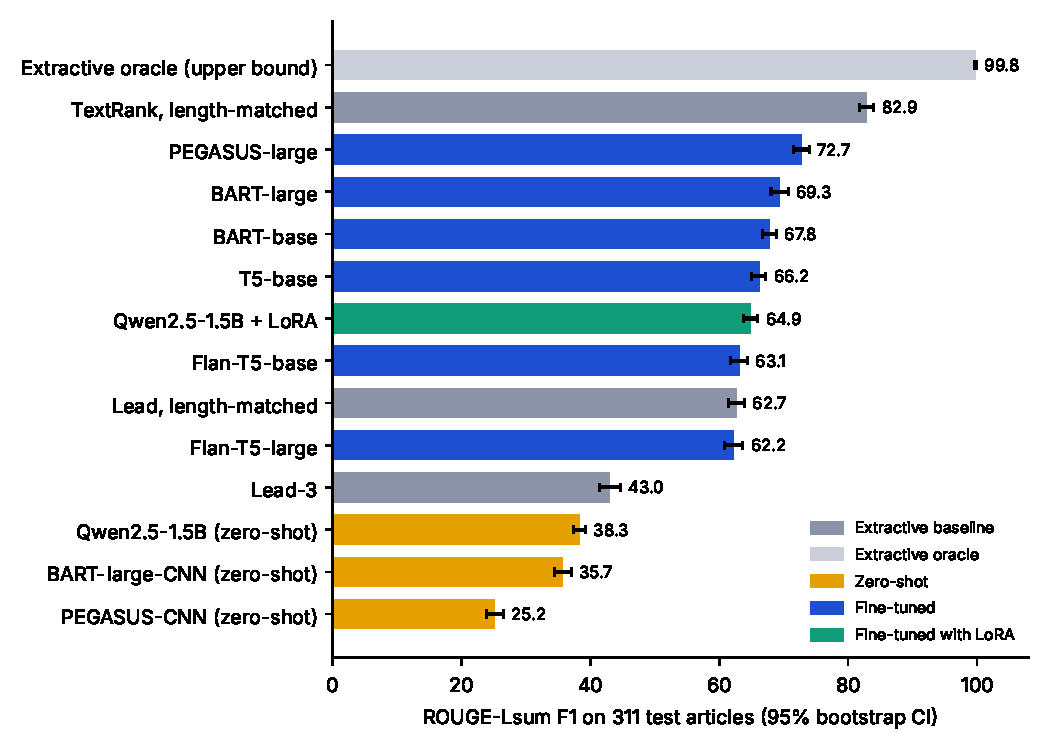
\includegraphics[width=0.78\linewidth]{figures/rouge_lsum_by_system.pdf}
\caption{ROUGE-Lsum by system with 95\% bootstrap intervals over the 311 test articles.}
\label{fig:main}
\end{figure}

\paragraph{TextRank is best.} The length-matched TextRank scores 82.9 ROUGE-Lsum. Against PEGASUS-large, the best fine-tuned model, the paired difference is $+10.2$ ROUGE-Lsum (95\% CI 8.7--11.5), $+12.7$ ROUGE-2 (11.0--14.4) and $+8.1$ BERTScore (6.6--9.6), and TextRank scores higher on 81\% of articles. The extractive oracle reaches 99.8, confirming that the references can be rebuilt almost exactly from article sentences.

\paragraph{Fine-tuned models.} PEGASUS-large is clearly the best trained model, followed by BART-large (69.3) and BART-base (67.8). All seven fine-tuned models beat the length-matched Lead baseline on ROUGE-2 (by 3.3 to 14.0 points, all intervals above zero), but on ROUGE-Lsum Flan-T5-base ($+0.4$, $-1.3$ to 2.0) and Flan-T5-large ($-0.5$, $-2.4$ to 1.3) are level with it. Larger models are not reliably better: BART-large improves on BART-base by 1.5 points, while Flan-T5-large scores below Flan-T5-base and has the largest variation across seeds (SD 2.8). The fine-tuned models copy heavily (coverage 0.99--1.00, 4--5\% novel bigrams) and rarely produce unsupported numbers ($\le$1.3\%).

\paragraph{Zero-shot models.} The CNN/DailyMail summarisers write 31--53 words, a third or less of the reference length, and score 25--36 ROUGE-Lsum. The zero-shot LLM writes about the requested length (149 words) but paraphrases (73\% novel bigrams, coverage 0.62) and scores 38.3; 7.8\% of the numbers it writes do not appear in the article. LoRA fine-tuning of the same model for about 70 minutes per seed on one T4 raises it to 64.9 and lowers unsupported numbers to 0.8\%.

\paragraph{Topic shift.} BART-base trained without a category lost 1.0 to 3.4 ROUGE-Lsum points on that category (Table~\ref{tab:xcat}); only for business does the interval exclude zero.

\begin{table}[t]
\centering\small
\caption{Held-out category. BART-base trained on four categories and tested on the fifth, against the same model trained on all categories (seed 0), on the same test articles. Difference with 95\% paired bootstrap CI.}
\label{tab:xcat}
\begin{tabular}{lrrrl}
\toprule
Held-out category & $n$ & In-domain R-Lsum & Held-out R-Lsum & Difference (CI)\\
\midrule
Business & 75 & 69.6 & 66.3 & $-3.4$ ($-5.9$, $-0.6$)\\
Entertainment & 55 & 67.8 & 66.8 & $-1.0$ ($-3.7$, 1.6)\\
Politics & 59 & 70.1 & 68.5 & $-1.6$ ($-4.0$, 0.7)\\
Sport & 73 & 66.0 & 63.5 & $-2.5$ ($-5.6$, 0.7)\\
Tech & 49 & 68.6 & 66.3 & $-2.3$ ($-5.2$, 0.8)\\
\bottomrule
\end{tabular}
\end{table}

\section{Discussion}\label{sec:discussion}
\paragraph{Why TextRank wins.} Two properties of the references explain the result. First, form: references are whole article sentences in article order, so a system that outputs whole sentences at the right length starts with an advantage. The fine-tuned models learned to copy (coverage $\ge$0.99) but stopped early, writing 96--160 words against the 179-word budget of the matched baselines; across systems, longer outputs generally scored higher, and the shortest writer, Flan-T5-large, came last among the fine-tuned models (Figure~\ref{fig:length}). Second, selection: length alone does not explain TextRank's score, because length-matched Lead, with the same budget, scores 20.2 points lower. TextRank's centrality ranking appears to agree with the rule that chose the reference sentences, which also favours, but is not limited to, early sentences (Figure~\ref{fig:position}).

\begin{figure}[t]
\centering
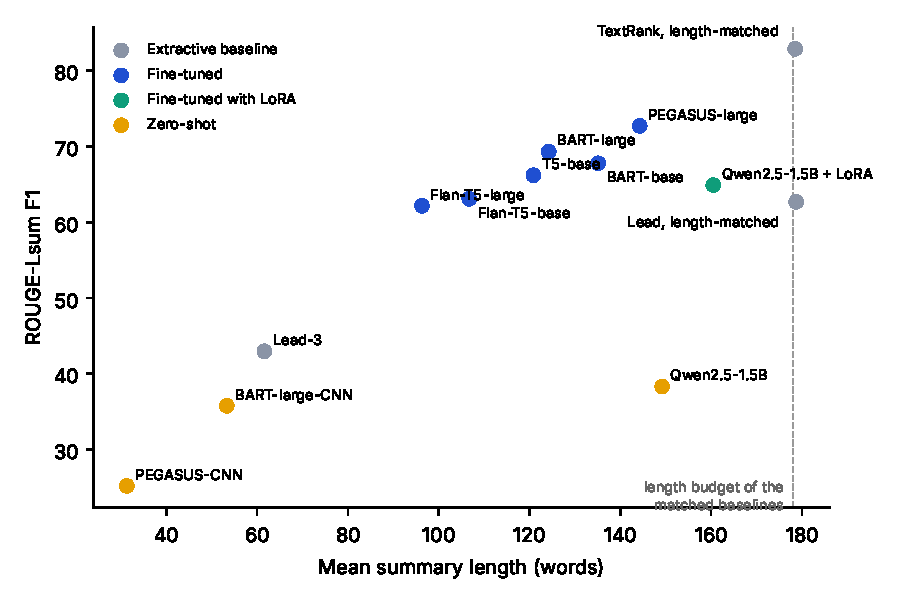
\includegraphics[width=0.7\linewidth]{figures/length_vs_rouge.pdf}
\caption{Mean summary length against ROUGE-Lsum. The dashed line marks the length budget of the matched extractive baselines.}
\label{fig:length}
\end{figure}

\paragraph{What the benchmark measures.} On this dataset a higher ROUGE score means a closer reproduction of one sentence-selection rule, not a better summary for a reader. This does not make PEGASUS worse than TextRank as a summariser; it means the benchmark cannot show which is better. For this dataset we recommend (i) de-duplicating before splitting and publishing the split, (ii) reporting a length-matched TextRank and Lead baseline next to any model, and (iii) controlling or reporting output length, since length differences of 50 words move ROUGE by several points.

\paragraph{Zero-shot LLMs.} A small instruction-tuned LLM used zero-shot is penalised twice: its free paraphrasing lowers overlap with extractive references, and it invents numbers. Reference-based metrics cannot tell these two effects apart; the unsupported-number rate separates them in part. Short in-domain LoRA fine-tuning removed most of both.

\section{Limitations}
The dataset is small (2,071 articles after de-duplication), from one publisher and two years. We report automatic metrics against a single reference per article; we did not run a human evaluation, and the unsupported-number rate is only a coarse check of factual errors. Hyperparameters were fixed rather than tuned, and output length of fine-tuned models was not controlled; length-aware decoding or tuning could narrow the gap to TextRank, though a 10-point difference is unlikely to close. The topic-shift experiment uses one model and one seed. Our inference about how the references were produced rests on their observable profile, not on documentation.

\section{Conclusion}
A training-free, length-matched TextRank outscores seven fine-tuned transformers, including a LoRA-tuned 1.5B LLM, on BBC News Summary, by 10 ROUGE-Lsum points over the best of them. The references are extracted sentences, about 45\% of each article, chosen in a way that TextRank's centrality ranking approximates. Results on this dataset should be read as agreement with that selection rule and reported against a length-matched TextRank baseline on a de-duplicated split.

\section*{Code and data availability}
Code (a tested Python package), the fixed split, all result tables, per-document scores and run records are available at \url{https://github.com/MHKhan50/NewsSum-Bench} and archived on Zenodo (doi:\href{https://doi.org/10.5281/zenodo.24046039}{10.5281/zenodo.24046039}) \cite{hussain2026newssum}. The full Kaggle run is public at \url{https://www.kaggle.com/code/muzammalhussain11/newssum-v2-bbc-news-summarisation-benchmark}. The seed-0 PEGASUS-large, BART-base and Qwen2.5-1.5B LoRA checkpoints are on Hugging Face (\url{https://huggingface.co/MHkhan50}), with a browser demo that runs TextRank and BART-base side by side (\url{https://huggingface.co/spaces/MHkhan50/newssum-demo}). The BBC articles are not redistributed.

\bibliographystyle{plainnat}
\bibliography{references}
\end{document}
